\hypertarget{javascript-hier}{%
\section{JavaScript hier}\label{javascript-hier}}

\begin{itemize}
\tightlist
\item
  Page web = HTML (+ CSS + JavaScript)
\item
  Exécuté par le browser (client)
\item
  Interprété, faiblement typé, OO
\item
  Historiquement

  \begin{itemize}
  \tightlist
  \item
    Depuis Netscape 2 (1995, Brendan Eich)
  \item
    Petites applications exécutées par le navigateur
  \item
    DHTML : rollovers, validation de formulaires, \ldots{}
  \end{itemize}
\end{itemize}

\hypertarget{javascript-aujourdhui}{%
\section{JavaScript aujourd'hui}\label{javascript-aujourdhui}}

\begin{itemize}
\tightlist
\item
  Page web = HTML + CSS + \textbf{JavaScript}
\item
  Compilation JIT
\item
  HTML5, AJAX, bookmarklets
\item
  One Page Apps
\item
  Implémentations hors-browser

  \begin{itemize}
  \tightlist
  \item
    Node.js, Spidermonkey, Rhino
  \item
    script d'app (Qt, Notepad++, \ldots{})
  \end{itemize}
\item
  Langage cible de compilateurs :
  \href{https://github.com/kripken/emscripten/wiki}{emscripten},
  \href{http://webassembly.org/}{WebAssembly}
\item
  Embarqué : \href{http://www.espruino.com/}{Espruino}
\end{itemize}

\hypertarget{script}{%
\section{*Script}\label{script}}

\begin{itemize}
\tightlist
\item
  ECMAScript : Norme depuis 1997

  \begin{itemize}
  \tightlist
  \item
    Juin 2017 :
    \href{https://www.ecma-international.org/publications/standards/Ecma-262.htm}{ECMA-262
    8th edition / 2017}
  \item
    \href{http://kangax.github.io/compat-table/es2016plus/}{Support} des
    différentes implémentations
  \item
    Conversions avec \href{https://babeljs.io/}{BabelJS}
  \end{itemize}
\item
  JavaScript : implémentation Firefox (réf. MDN)
\item
  Variantes (à transpiler) :

  \begin{itemize}
  \tightlist
  \item
    \href{https://www.typescriptlang.org/}{Typescript} : variante
    fortement typée, avec des classes (MS)
  \item
    \href{http://coffeescript.org/}{Coffescript}

    \begin{itemize}
    \tightlist
    \item
      sucre syntaxique
    \item
      compilé -\textgreater{} js
    \end{itemize}
  \end{itemize}
\end{itemize}

\hypertarget{javascript}{%
\section{JavaScript}\label{javascript}}

\begin{itemize}
\tightlist
\item
  Différentes
  \href{https://en.wikipedia.org/wiki/List_of_ECMAScript_engines}{implémentations}
  : navigateur, srv, apps, \ldots{}
\item
  Permissif : du mauvais code est peu maintenable

  \begin{itemize}
  \tightlist
  \item
    \href{https://addyosmani.com/resources/essentialjsdesignpatterns/book/}{Design
    Patterns}
  \item
    \href{http://jstherightway.org/}{Bonnes pratiques}
  \end{itemize}
\item
  Interface pour scripter le navigateur

  \begin{itemize}
  \tightlist
  \item
    Accès et modification du contenu via DOM
  \item
    \href{http://www.howtogeek.com/125846/the-most-useful-bookmarklets-to-enhance-your-browsing-experience/}{Bookmarklets},
    \href{http://www.hongkiat.com/blog/100-useful-bookmarklets-for-better-productivity-ultimate-list/}{exemples}
  \item
    Requêtes HTTP (Xml Http Request)
  \end{itemize}
\item
  Développement d'applications complètes, parfois offline
\item
  Langage de script généraliste (paquets npm)
\end{itemize}

\hypertarget{caractuxe9ristiques-du-langage}{%
\section{Caractéristiques du
langage}\label{caractuxe9ristiques-du-langage}}

\begin{itemize}
\tightlist
\item
  Orienté Objet par prototype
\item
  Syntaxe proche de C, Java
\item
  Faiblement typé :

  \begin{itemize}
  \tightlist
  \item
    Pas de déclaration, type déterminé par la dernière affectation
  \item
    Risque : typo =\textgreater{} nouvelle variable. Utiliser
    \begin{otherlanguage}{english}\texttt{var}\end{otherlanguage}
  \end{itemize}
\item
  Types :

  \begin{itemize}
  \tightlist
  \item
    Primitifs :
    \begin{otherlanguage}{english}\texttt{Boolean\ Null\ Undefined\ Number\ String\ Symbol}\end{otherlanguage}
  \item
    Objets :
    \begin{otherlanguage}{english}\texttt{Object\ Function}\end{otherlanguage}
  \end{itemize}
\item
  Particularités

  \begin{itemize}
  \tightlist
  \item
    \href{https://developer.mozilla.org/fr/docs/Web/JavaScript/Guide/Le_mod\%C3\%A8le_objet_JavaScript_en_d\%C3\%A9tails}{Prototypes}
  \item
    \href{http://www.w3schools.com/js/js_function_closures.asp}{Fermetures}
  \item
    \href{https://www.promisejs.org/}{Promesses}
    (\href{https://developer.mozilla.org/en/docs/Web/JavaScript/Reference/Global_Objects/Promise}{MDN},
    \href{https://developers.google.com/web/fundamentals/getting-started/primers/promises}{Google})
  \end{itemize}
\end{itemize}

\hypertarget{fonctions}{%
\section{Fonctions}\label{fonctions}}

\begin{itemize}
\tightlist
\item
  Pas de type de retour
\item
  Possibilité de retourner ou non une valeur
\item
  Sans retour, valeur spéciale : undefined
\item
  Pas de surcharge (la dernière définie prime)
\item
  function est un type
\item
  Fonctions imbriquées, anonymes
\item
  Fonctions globales :
\end{itemize}

\begin{otherlanguage}{english}

\begin{Shaded}
\begin{Highlighting}[]
\AttributeTok{escape}\NormalTok{()}\OperatorTok{,} \AttributeTok{unescape}\NormalTok{()}\OperatorTok{,} \AttributeTok{isFinite}\NormalTok{()}\OperatorTok{,} \AttributeTok{isNaN}\NormalTok{()}\OperatorTok{,}
\AttributeTok{parseFloat}\NormalTok{()}\OperatorTok{,} \AttributeTok{parseInt}\NormalTok{()}\OperatorTok{,} \AttributeTok{Number}\NormalTok{()}\OperatorTok{,} \AttributeTok{String}\NormalTok{()}\OperatorTok{,} 
\AttributeTok{eval}\NormalTok{()}\OperatorTok{,}\NormalTok{ ...}
\end{Highlighting}
\end{Shaded}

\end{otherlanguage}

\hypertarget{javascript-dans-la-page-web}{%
\section{JavaScript dans la page
web}\label{javascript-dans-la-page-web}}

\begin{itemize}
\tightlist
\item
  Éléments
  \begin{otherlanguage}{english}\texttt{\textless{}script\textgreater{}}\end{otherlanguage}
  exécutés dans l'ordre de la page
\item
  Conseillé de les placer en
  \href{https://developer.yahoo.com/performance/rules.html\#js_bottom=}{fin
  de page}
\item
  Evénements (onclick, onerror, onsubmit, \ldots{})

  \begin{itemize}
  \tightlist
  \item
    Embarqués dans les balises (onXXX)
  \end{itemize}
\end{itemize}

\begin{otherlanguage}{english}

\begin{Shaded}
\begin{Highlighting}[]
\KeywordTok{<div}\OtherTok{ id=}\StringTok{"intro"}\OtherTok{ onclick=}\StringTok{"change();"} \KeywordTok{/>}
\end{Highlighting}
\end{Shaded}

\end{otherlanguage}

\begin{otherlanguage}{english}

\end{otherlanguage}

\begin{otherlanguage}{english}

\end{otherlanguage}

\begin{otherlanguage}{english}

\end{otherlanguage}

Utiliser DOM

\begin{otherlanguage}{english}

\end{otherlanguage}

\begin{otherlanguage}{english}

\end{otherlanguage}

\begin{otherlanguage}{english}

\end{otherlanguage}

\begin{otherlanguage}{english}

\begin{Shaded}
\begin{Highlighting}[]
\KeywordTok{<script}\OtherTok{ type=}\StringTok{"text/javascript"}\KeywordTok{>}
\end{Highlighting}
\end{Shaded}

\end{otherlanguage}

\begin{otherlanguage}{english}

\begin{Shaded}
\begin{Highlighting}[]
    \VariableTok{document}\NormalTok{.}\AttributeTok{getElementById}\NormalTok{(}\StringTok{"intro"}\NormalTok{).}\AttributeTok{onclick} \OperatorTok{=}\NormalTok{ change}\OperatorTok{;}
\end{Highlighting}
\end{Shaded}

\end{otherlanguage}

\begin{otherlanguage}{english}

\begin{Shaded}
\begin{Highlighting}[]
\KeywordTok{</script>}
\end{Highlighting}
\end{Shaded}

\end{otherlanguage}

\begin{itemize}
\tightlist
\item
  Conseillé d'inclure le code (attribut src)
\end{itemize}

\begin{otherlanguage}{english}

\begin{Shaded}
\begin{Highlighting}[]
\KeywordTok{<script}\OtherTok{ type=}\StringTok{"text/javascript"}\OtherTok{ src=}\StringTok{"script02.js"}\KeywordTok{></script>} 
\end{Highlighting}
\end{Shaded}

\end{otherlanguage}

\begin{otherlanguage}{english}\texttt{language="JavaScript"}\end{otherlanguage}
est déprécié et
\begin{otherlanguage}{english}\texttt{type}\end{otherlanguage} vaut par
défaut
\begin{otherlanguage}{english}\texttt{text/javascript}\end{otherlanguage}.

\begin{quote}
The type attribute gives the language of the script or format of the
data. {[}\ldots{}{]} The default, which is used if the attribute is
absent, is ``text/javascript''.

\href{https://www.w3.org/TR/html5/scripting-1.html\#the-script-element}{HTML5:
script}
\end{quote}

\hypertarget{unobstrusive-js}{%
\section{\texorpdfstring{\href{https://en.wikipedia.org/wiki/Unobtrusive_JavaScript}{Unobstrusive
JS}}{Unobstrusive JS}}\label{unobstrusive-js}}

\begin{itemize}
\tightlist
\item
  Séparation JS\ldots{}
\end{itemize}

\begin{otherlanguage}{english}

\begin{Shaded}
\begin{Highlighting}[]
\VariableTok{document}\NormalTok{.}\AttributeTok{addEventListener}\NormalTok{(}\StringTok{"DOMContentLoaded"}\OperatorTok{,} \KeywordTok{function}\NormalTok{() }\OperatorTok{\{}
    \VariableTok{document}\NormalTok{.}\AttributeTok{getElementById}\NormalTok{(}\StringTok{'date'}\NormalTok{).}\AttributeTok{addEventListener}\NormalTok{(}\StringTok{"change"}\OperatorTok{,}\NormalTok{ validateDate)}\OperatorTok{;}
\OperatorTok{\};}
\end{Highlighting}
\end{Shaded}

\end{otherlanguage}

\begin{itemize}
\tightlist
\item
  \ldots{}et HTML
\end{itemize}

\begin{otherlanguage}{english}

\begin{Shaded}
\begin{Highlighting}[]
    \KeywordTok{<input}\OtherTok{ type=}\StringTok{"text"}\OtherTok{ name=}\StringTok{"date"}\OtherTok{ id=}\StringTok{"date"} \KeywordTok{/>}
\end{Highlighting}
\end{Shaded}

\end{otherlanguage}

\begin{itemize}
\tightlist
\item
  Dégradation élégante

  \begin{itemize}
  \tightlist
  \item
    Alternatives pour un browser ne supportant pas JS
  \end{itemize}
\item
  Accessibilité

  \begin{itemize}
  \tightlist
  \item
    Les fonctionnalités restent accessibles en cas d'erreur
  \end{itemize}
\item
  Utilisabilité

  \begin{itemize}
  \tightlist
  \item
    Le script doit faire gagner du temps, pas distraire
  \end{itemize}
\end{itemize}

\begin{quote}
It is an incredibly popular mistake to use
\begin{otherlanguage}{english}\texttt{load}\end{otherlanguage} where
\begin{otherlanguage}{english}\texttt{DOMContentLoaded}\end{otherlanguage}
would be much more appropriate, so be cautious.

\href{https://developer.mozilla.org/en/docs/Web/Events/DOMContentLoaded}{MDN:
DOMContentLoaded}
\end{quote}

\hypertarget{node.js}{%
\section{\texorpdfstring{\href{https://nodejs.org}{Node.js}}{Node.js}}\label{node.js}}

\begin{itemize}
\tightlist
\item
  Node.js : une implémentation hors navigateur

  \begin{itemize}
  \tightlist
  \item
    environnement d'exécution + bibliothèques
  \item
    event driven, non-blocking IO -\textgreater{} scalable
  \item
    V8 engine
  \item
    scripts exécutables sans navigateur
  \item
    \href{https://www.npmjs.com}{npm} : gestionnaire de paquets
  \item
    gulp : make js
  \end{itemize}
\item
  \href{https://docs.google.com/spreadsheets/d/1LyRwn6E8k7NM5bw2hJ7pWD7BWjgN_EskQ0ZMNphrffE}{Exemples}
  d'applications

  \begin{itemize}
  \tightlist
  \item
    gulp, grunt, bower, yarn
  \item
    browserify
  \item
    serveur http
  \item
    express, cordova, forever, dev, pm2, karma, sails
  \end{itemize}
\item
  \href{https://www.tutorialspoint.com/nodejs/index.htm}{Tuto},
  \href{https://runkit.com}{Playground}
\end{itemize}

\hypertarget{dom}{%
\section{DOM}\label{dom}}

\begin{itemize}
\tightlist
\item
  Document Object Model
\item
  Représentation arborescente de la page
\item
  Accessible depuis objet JS document
\item
  Possibilité d'accéder au contenu de la page :

  \begin{itemize}
  \tightlist
  \item
    Lecture
  \item
    Modification
  \item
    Ajout
  \end{itemize}
\item
  JS peut donc modifier le contenu d'une page
\end{itemize}

\hypertarget{dom-1}{%
\section{DOM}\label{dom-1}}

\begin{otherlanguage}{english}

\begin{Shaded}
\begin{Highlighting}[]
\KeywordTok{<html>}
\KeywordTok{<head>}
   \KeywordTok{<title>}\NormalTok{My title}\KeywordTok{</title>}
\KeywordTok{</head>}
\KeywordTok{<body>}
    \KeywordTok{<h1>}\NormalTok{A heading}\KeywordTok{</h1>}
    \KeywordTok{<a}\OtherTok{ href=}\StringTok{"#"}\KeywordTok{>}\NormalTok{Link text}\KeywordTok{</a>}
\KeywordTok{</body>}
\KeywordTok{</html>}
\end{Highlighting}
\end{Shaded}

\end{otherlanguage}

\begin{figure}
\centering
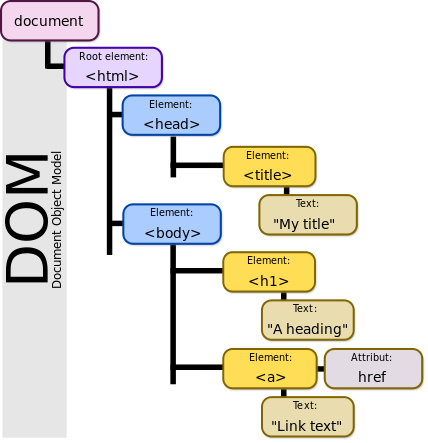
\includegraphics{src/img/DOM-model.png}
\caption{DOM tree}
\end{figure}

\begin{otherlanguage}{english}

\end{otherlanguage}

\begin{otherlanguage}{english}

\end{otherlanguage}

\hypertarget{lobjet-document}{%
\section{L'objet Document}\label{lobjet-document}}

\begin{itemize}
\tightlist
\item
  Trouver ou modifier des éléments
\item
  Méthodes de
  \begin{otherlanguage}{english}\texttt{Document}\end{otherlanguage}
\end{itemize}

\begin{otherlanguage}{english}

\begin{Shaded}
\begin{Highlighting}[]
    \AttributeTok{getElementById}\NormalTok{()}\OperatorTok{,} \AttributeTok{getElementsByTagName}\NormalTok{()}\OperatorTok{,} \AttributeTok{getElementByClass}\NormalTok{()}\OperatorTok{,}  
    \AttributeTok{createElement}\NormalTok{()}\OperatorTok{,} \AttributeTok{createTextNode}\NormalTok{()}
\end{Highlighting}
\end{Shaded}

\end{otherlanguage}

\begin{itemize}
\tightlist
\item
  Méthodes de
  \begin{otherlanguage}{english}\texttt{Node}\end{otherlanguage} (appel
  depuis nœud parent)
\end{itemize}

\begin{otherlanguage}{english}

\begin{Shaded}
\begin{Highlighting}[]
    \AttributeTok{insertBefore}\NormalTok{(child)}\OperatorTok{,} \AttributeTok{appendChild}\NormalTok{(child)}\OperatorTok{,}
    \AttributeTok{removeChild}\NormalTok{(child)}\OperatorTok{,} \AttributeTok{replaceChild}\NormalTok{(}\KeywordTok{new}\OperatorTok{,}\NormalTok{old)}
\end{Highlighting}
\end{Shaded}

\end{otherlanguage}

\hypertarget{ajouter-un-noeud}{%
\section{Ajouter un noeud}\label{ajouter-un-noeud}}

\begin{otherlanguage}{english}

\begin{Shaded}
\begin{Highlighting}[]
\KeywordTok{function} \AttributeTok{addNode}\NormalTok{() }\OperatorTok{\{}
     \KeywordTok{var}\NormalTok{ inText }\OperatorTok{=} \VariableTok{document}\NormalTok{.}\AttributeTok{getElementById}\NormalTok{(}\StringTok{"textArea"}\NormalTok{).}\AttributeTok{value}\OperatorTok{;}
     \KeywordTok{var}\NormalTok{ newText }\OperatorTok{=} \VariableTok{document}\NormalTok{.}\AttributeTok{createTextNode}\NormalTok{(inText)}\OperatorTok{;}

     \KeywordTok{var}\NormalTok{ newGraf }\OperatorTok{=} \VariableTok{document}\NormalTok{.}\AttributeTok{createElement}\NormalTok{(}\StringTok{"p"}\NormalTok{)}\OperatorTok{;}
     \VariableTok{newGraf}\NormalTok{.}\AttributeTok{appendChild}\NormalTok{(newText)}\OperatorTok{;}

     \KeywordTok{var}\NormalTok{ docBody }\OperatorTok{=} \VariableTok{document}\NormalTok{.}\AttributeTok{getElementsByTagName}\NormalTok{(}\StringTok{"body"}\NormalTok{)[}\DecValTok{0}\NormalTok{]}\OperatorTok{;}
     \VariableTok{docBody}\NormalTok{.}\AttributeTok{appendChild}\NormalTok{(newGraf)}\OperatorTok{;}
\OperatorTok{\}}
\end{Highlighting}
\end{Shaded}

\end{otherlanguage}

\begin{itemize}
\tightlist
\item
  Création du nouveau nœud :

  \begin{itemize}
  \tightlist
  \item
    \begin{otherlanguage}{english}\texttt{newText}\end{otherlanguage}
    contient le texte à ajouter
  \item
    \begin{otherlanguage}{english}\texttt{newGraf}\end{otherlanguage}
    est un élément
    \begin{otherlanguage}{english}\texttt{p}\end{otherlanguage} qui
    contient le texte
  \end{itemize}
\item
  Ajout du nœud comme une feuille de body :

  \begin{itemize}
  \tightlist
  \item
    Sélection du parent (le premier noeud
    \begin{otherlanguage}{english}\texttt{body}\end{otherlanguage})
  \item
    Ajout du nouveau nœud depuis son parent
  \end{itemize}
\end{itemize}

\hypertarget{supprimer-un-nux153ud}{%
\section{Supprimer un nœud}\label{supprimer-un-nux153ud}}

\begin{otherlanguage}{english}

\begin{Shaded}
\begin{Highlighting}[]
\KeywordTok{function} \AttributeTok{delNode}\NormalTok{() }\OperatorTok{\{}
   \KeywordTok{var}\NormalTok{ allGrafs }\OperatorTok{=} \VariableTok{document}\NormalTok{.}\AttributeTok{getElementsByTagName}\NormalTok{(}\StringTok{"p"}\NormalTok{)}\OperatorTok{;}

   \ControlFlowTok{if}\NormalTok{ (}\VariableTok{allGrafs}\NormalTok{.}\AttributeTok{length} \OperatorTok{>} \DecValTok{1}\NormalTok{) }\OperatorTok{\{}
      \KeywordTok{var}\NormalTok{ lastGraf }\OperatorTok{=} \VariableTok{allGrafs}\NormalTok{.}\AttributeTok{item}\NormalTok{ (}\VariableTok{allGrafs}\NormalTok{.}\AttributeTok{length}\DecValTok{-1}\NormalTok{)}\OperatorTok{;}
      \VariableTok{lastGraf}\NormalTok{.}\VariableTok{parentNode}\NormalTok{.}\AttributeTok{removeChild}\NormalTok{(lastGraf)}\OperatorTok{;}
   \OperatorTok{\}}
   \ControlFlowTok{else} \OperatorTok{\{}
      \VariableTok{console}\NormalTok{.}\AttributeTok{error}\NormalTok{(}\StringTok{"Nothing to remove!"}\NormalTok{)}\OperatorTok{;}
   \OperatorTok{\}}
\OperatorTok{\}}
\end{Highlighting}
\end{Shaded}

\end{otherlanguage}

\begin{itemize}
\tightlist
\item
  Sélection du nœud à supprimer :

  \begin{itemize}
  \tightlist
  \item
    \begin{otherlanguage}{english}\texttt{allGrafs}\end{otherlanguage}
    contient tous les éléments
    \begin{otherlanguage}{english}\texttt{p}\end{otherlanguage}
  \item
    \begin{otherlanguage}{english}\texttt{lastGraf}\end{otherlanguage}
    contient le denier du tableau
    \begin{otherlanguage}{english}\texttt{allGrafs}\end{otherlanguage}
  \end{itemize}
\item
  Suppression :

  \begin{itemize}
  \tightlist
  \item
    Suppression du nœud sélectionné depuis son
    \href{https://developer.mozilla.org/en-US/docs/Web/API/Node/parentNode}{parent}
  \end{itemize}
\end{itemize}

\hypertarget{insuxe9rer-un-nux153ud}{%
\section{Insérer un nœud}\label{insuxe9rer-un-nux153ud}}

\begin{otherlanguage}{english}

\begin{Shaded}
\begin{Highlighting}[]
\KeywordTok{function} \AttributeTok{insertNode}\NormalTok{() }\OperatorTok{\{}
     \KeywordTok{var}\NormalTok{ newText }\OperatorTok{=} \VariableTok{document}\NormalTok{.}\AttributeTok{createTextNode}\NormalTok{(}\StringTok{"New Text"}\NormalTok{)}\OperatorTok{;}
     \KeywordTok{var}\NormalTok{ newGraf }\OperatorTok{=} \VariableTok{document}\NormalTok{.}\AttributeTok{createElement}\NormalTok{(}\StringTok{"p"}\NormalTok{)}\OperatorTok{;}
     \VariableTok{newGraf}\NormalTok{.}\AttributeTok{appendChild}\NormalTok{(newText)}\OperatorTok{;}
    
     \KeywordTok{var}\NormalTok{ divMod }\OperatorTok{=} \VariableTok{document}\NormalTok{.}\AttributeTok{getElementsByTagName}\NormalTok{(}\StringTok{"div"}\NormalTok{)[}\DecValTok{0}\NormalTok{]}\OperatorTok{;}
     \KeywordTok{var}\NormalTok{ allGrafs }\OperatorTok{=} \VariableTok{divMod}\NormalTok{.}\AttributeTok{getElementsByTagName}\NormalTok{(}\StringTok{"p"}\NormalTok{)}\OperatorTok{;}
     \KeywordTok{var}\NormalTok{ oldGraf }\OperatorTok{=} \VariableTok{allGrafs}\NormalTok{.}\AttributeTok{item}\NormalTok{(}\DecValTok{0}\NormalTok{)}\OperatorTok{;}             \CommentTok{// position}

     \VariableTok{divMod}\NormalTok{.}\AttributeTok{insertBefore}\NormalTok{(newGraf}\OperatorTok{,}\NormalTok{oldGraf)}\OperatorTok{;}
\OperatorTok{\}}
\end{Highlighting}
\end{Shaded}

\end{otherlanguage}

\begin{itemize}
\tightlist
\item
  Création du nouveau nœud :

  \begin{itemize}
  \tightlist
  \item
    \begin{otherlanguage}{english}\texttt{allGrafs}\end{otherlanguage}
    contient tous les éléments
    \begin{otherlanguage}{english}\texttt{p}\end{otherlanguage}
  \item
    \begin{otherlanguage}{english}\texttt{lastGraf}\end{otherlanguage}
    contient le denier du tableau
    \begin{otherlanguage}{english}\texttt{allGrafs}\end{otherlanguage}
  \end{itemize}
\item
  Insertion :

  \begin{itemize}
  \tightlist
  \item
    Recherche du parent
  \item
    Recherche du frère gauche
  \item
    Insertion depuis le parent
  \end{itemize}
\end{itemize}

\hypertarget{avec-jquery}{%
\section{Avec jQuery}\label{avec-jquery}}

\begin{itemize}
\tightlist
\item
  Création et ajout :
\end{itemize}

\begin{otherlanguage}{english}

\begin{Shaded}
\begin{Highlighting}[]
    \KeywordTok{var}\NormalTok{ noeud }\OperatorTok{=} \AttributeTok{$}\NormalTok{(}\StringTok{'<p>Nouveau texte</p>'}\NormalTok{)}\OperatorTok{;}  \CommentTok{// create node}
    \AttributeTok{$}\NormalTok{(}\StringTok{"body"}\NormalTok{).}\AttributeTok{append}\NormalTok{(noeud)}\OperatorTok{;}                \CommentTok{// après le dernier fils}
\end{Highlighting}
\end{Shaded}

\end{otherlanguage}

\begin{itemize}
\tightlist
\item
  Sélection et Suppression :
\end{itemize}

\begin{otherlanguage}{english}

\begin{Shaded}
\begin{Highlighting}[]
    \KeywordTok{var}\NormalTok{ noeud }\OperatorTok{=} \AttributeTok{$}\NormalTok{(}\StringTok{"p"}\NormalTok{)}\OperatorTok{;} \CommentTok{// select node(s)}
    \VariableTok{noeud}\NormalTok{.}\AttributeTok{remove}\NormalTok{()}\OperatorTok{;}
\end{Highlighting}
\end{Shaded}

\end{otherlanguage}

\hypertarget{ruxe9fuxe9rences}{%
\section{Références}\label{ruxe9fuxe9rences}}

\begin{itemize}
\tightlist
\item
  Une
  \href{https://developer.mozilla.org/fr/docs/Web/JavaScript/Une_r\%C3\%A9introduction_\%C3\%A0_JavaScript}{réintroduction
  à JavaScript}
\item
  \href{https://hackernoon.com/how-it-feels-to-learn-javascript-in-2016-d3a717dd577f}{How
  does it feel to learn JS in 2016}
\item
  Référence
  \href{https://developer.mozilla.org/fr/docs/Web/JavaScript/Reference}{MDN}
\item
  Tutoriels \href{http://www.w3schools.com/js/}{w3schools}
\item
  Outils de développement Chrome et Firefox (Ctrl+Shift I)
\item
  Firefox :

  \begin{itemize}
  \tightlist
  \item
    \href{https://addons.mozilla.org/fr/firefox/addon/tilt/}{Tilt3D}
    (Ctrl+Shift+L)
  \item
    Barre développement (Shift+F2)
  \end{itemize}
\item
  Outils web

  \begin{itemize}
  \tightlist
  \item
    \href{https://jsfiddle.net/}{JSFiddle}
  \item
    \href{http://www.jslint.com/}{JSLint}
  \end{itemize}
\end{itemize}

\begin{otherlanguage}{english}

\end{otherlanguage}

\begin{otherlanguage}{english}

\end{otherlanguage}

\hypertarget{sources}{%
\section{Sources}\label{sources}}
